%**********************************************************
\subsection{Task Overview}
One can define and describe briefly how the gateway is implemented, making use of threads and processes.

\begin{itemize}
	\item \textbf{tLoraRecv: } receives all messages from local systems, using LoRa communication;
	\item \textbf{tTCPRecv: } receives all messages from the remote server, using TCP-IP communication;	
	\item \textbf{LoraComm::tSend: } sends all received messages from the remote server, in textit{tTCPRecv}, to the local systems, using LoRa communication; private method of the LoraComm class;
	\item \textbf{TCPclient::tSend: } sends all received messages from local systems, in \textit{tLoraRecv}, to the remote server, using TCP-IP communication; private method of the TCPclient class.
\end{itemize}

One can define the relationship between the tasks as follows, in figure \ref{fig:GwOverview}. To communicate the local system received messages and the remote server sender service its used a vector of messages, named \textit{msgs\_to\_rs}. In the communication between the remote server received messages and the local system sender service its also used a vector of messages, named \textit{msgs\_to\_ls}.

\begin{figure}[H]
	\centering
	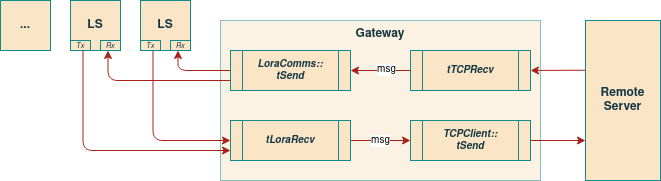
\includegraphics[width=1\textwidth]{09sw_specification/GwOverview}
	\caption{Gateway Overview.}
	\label{fig:GwOverview}
\end{figure}

%**********************************************************
\clearpage
\subsection{Task Priority}
The priority assignment diagram for the gateway is represented in figure \ref{fig:gwt_priority}.

\begin{figure}[H]
	\centering
	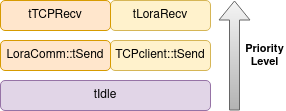
\includegraphics[width=0.5\textwidth]{09sw_specification/GwPriority}
	\caption{Gateway Priority Assignment Schematic.}
	\label{fig:gwt_priority}
\end{figure}

%**********************************************************
\subsection{Task Synchronization}

\myparagraph{Condition Variables}
The condition variables used in this system are listed below.

\begin{itemize}
	\item \textbf{LoraComm::condSend:} used to notify \textit{tLoraSend} that a new message is ready to be sent; private member of class LoraComm;
	\item \textbf{TCPclient::condSend:} used to notify \textit{tTCPSend} that a new message is ready to be sent; private member of class TCPclient.
\end{itemize}

\myparagraph{Mutexes}
The mutexes used in this system are listed bellow, which are all private members of LoraComm and TCPclient classes.

\begin{itemize}
	\item \textbf{LoraComm::mutComm:} used to protect the LoRa communications (send and receive);
	\item \textbf{LoraComm::mutSend:}	used to protect the handling of the vector \textit{msgs\_to\_ls};
	
	\item \textbf{TCPclient::mutComm:} used to protect the TCP/IP communications (send and receive);
	\item \textbf{TCPclient::mutSend:} used to protect the handling of the vector \textit{msgs\_to\_rs}.
\end{itemize}

%\subsection{Task Communication}
%In order to communicate all messages between the LoRa related tasks and the TCP related tasks are used two vectors of strings, \textit{msgs\_to\_rs} and \textit{msgs\_to\_ls}. This belongs to the container library \textit{std::vector} from C++ libraries, which implements a dynamic contiguous array. The storage of the vector is handled automatically being expanded and contracted as needed. This provides functions like \textit{push\_back()}, \textit{insert()} or \textit{pop\_back()} which allows to insert or remove new elements as needed.

%**********************************************************
\subsection{Class Diagrams}
In figure \ref{fig:GwclassDiag} is represented the class diagram of gateway. The class \textit{CGateway} is the main class of the system that initializes the objects of each class listed below.

\begin{itemize}
	\item \textbf{CLoraComm:} manages the LoRa communications, interfacing with the LoRa module;
	
	\item \textbf{CTCPclient:} manages the TCP-IP communication with the remote server;
\end{itemize}

\begin{figure}[H]
	\centering
	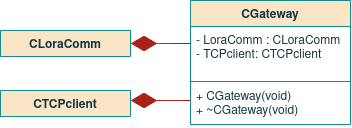
\includegraphics[width=.8\textwidth]{09sw_specification/GwClassDiagram}
	\caption{Gateway Class Diagram.}
	\label{fig:GwclassDiag}
\end{figure}

\myparagraph{Class CTCPclient}

In figure \ref{fig:TCPclient} is shown the TCPclient class. This class defines a TCPclient capable of establishing a connection to a given remote server and to exchange messages to it, via TCP-IP. Like in the LoraComm class, which is very similar to this, its used a vector of strings, \textit{tx\_msgs} to store messages, providing a waiting list of messages to be sent.

\begin{figure}[H]
	\centering
	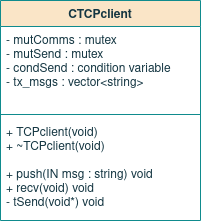
\includegraphics[width=.5\textwidth]{09sw_specification/TCPclientClass}
	\caption{Class Diagram: TCPclient.}
	\label{fig:TCPclientClass}
\end{figure}

A TCPclient can be created through the use of the constructor, shown in figure \ref{fig:TCPclient}. This connects to a given server, defined by the string \textit{host}, and to the port \textit{port}, via TCP-IP and initializes all the private members.

\begin{figure}[H]
	\centering
	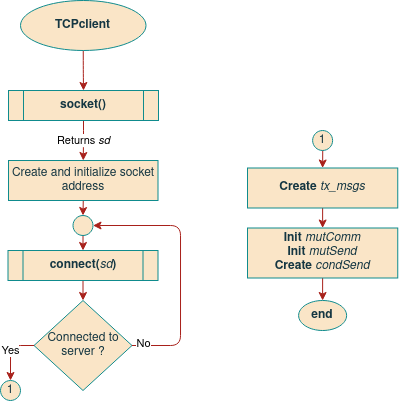
\includegraphics[width=.8\textwidth]{09sw_specification/TCPclient}
	\caption{Class Diagram: TCPclient construtor.}
	\label{fig:TCPclient}
\end{figure}

A message can be put in the waiting list to be sent through the use of \textit{TCPclient.push(msg)}, as shown in figure \ref{fig:TCPclientPush}. As in the LoraComm class, this function is responsible for adding a message to the \textit{tx\_msgs} vector and signal the condition variable \textit{condSend} for the task \textit{tSend} to send the message.

\begin{figure}[H]
	\centering
	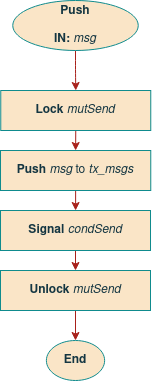
\includegraphics[width=.3\textwidth]{09sw_specification/TCPclientPush}
	\caption{Class Diagram: TCPclient Push method.}
	\label{fig:TCPclientPush}
\end{figure}

In order to send a message, this class has a built-in thread, \textit{tSend} that is created through the use of \textit{TCPclient.run()}, as shown in figure \ref{fig:TCPclientRun}.

\begin{figure}[H]
	\centering
	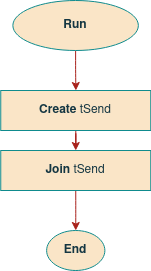
\includegraphics[width=.3\textwidth]{09sw_specification/TCPclientRun}
	\caption{Class Diagram: TCPclient Run method.}
	\label{fig:TCPclientRun}
\end{figure}

To send a message to the server, the thread \textit{tSend}, works similarly to \textit{LoraComm::tSend}, apart from the function used to send the message to the destination, that in this case is the \textit{send()} function, for TCP-IP. The flowchart for this method is presented in figure \ref{fig:TCPclientSend}.

\begin{figure}[H]
	\centering
	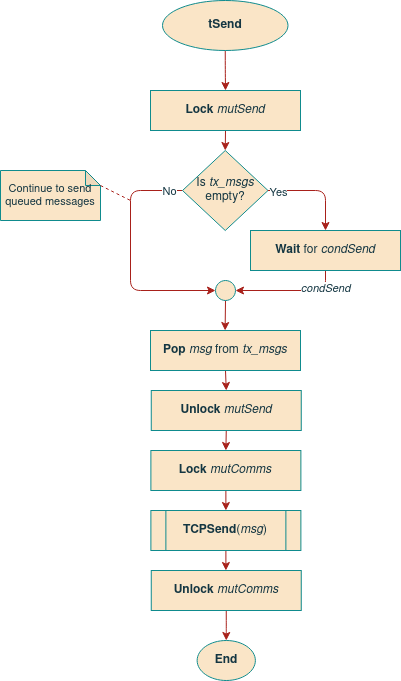
\includegraphics[width=.8\textwidth]{09sw_specification/TCPclientSend}
	\caption{Class Diagram: TCPclient tSend thread.}
	\label{fig:TCPclientSend}
\end{figure}

To receive a message from the server, in a non blocking mode, there is the method \textit{recv()}, presented in figure \ref{fig:TCPclientRecv}.

\begin{figure}[H]
	\centering
	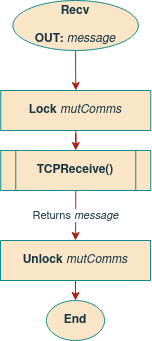
\includegraphics[width=.3\textwidth]{09sw_specification/TCPclientRecv}
	\caption{Class Diagram: TCPclient Recv method.}
	\label{fig:TCPclientRecv}
\end{figure}

%**********************************************************
\subsection{Flowcharts}
Each local system has a predefined ID, which may be presented in a physical label for an operator to use this information. When a local system is being installed, it will use it's predefined ID in all communications with the remote server until the operator registers the local system that's being installed, in the remote server. By doing this, the remote server assigns a new ID to the local system, which is then sent to the local system, for this to be used in further communications.

\myparagraph{tLoraRecv}

This task, presented in figure \ref{fig:gwtLoraRecv}, is responsible for receiving all the packets sent by the local systems, through LoRa communication, using \textit{LoraComm.recv()} function, that was already detailed.

When a message is received it is pushed into the TCP client list of queue messages, waiting to be sent to the remote server.

\begin{figure}[H]
	\centering
	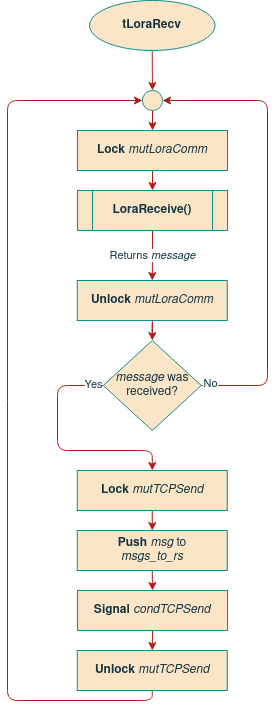
\includegraphics[width=.5\textwidth]{09sw_specification/gwtLoraRecv}
	\caption{Flowchart: Gateway tLoraRecv.}
	\label{fig:gwtLoraRecv}
\end{figure}

%\myparagraph{tLoraSend}
%
%This task, presented in figure \ref{fig:gwtLoraSend}, is responsible for sending all the packets sent by the remote system to the local systems. In addiction to the mutex \textit{mutLoraComm}, this task makes use of another mutex \textit{mutLoraSend}, which comes along with the condition variable \textit{condLoraSend}, in order to protect the insertion and removal of messages from the vector \textit{msgs\_to\_ls}.
%
%When there are no messages to send to the local systems, i.e, the messages vector \textit{msgs\_to\_ls} is empty, then the task enters a sleep state, waiting for \textit{condLoraSend} to be notified. When this happens, the mutex that protects LoRa communication is locked and a message is popped from the queue of messages to being sent to the local systems. If the vector \textit{msgs\_to\_ls} is not empty after sending a message, this task continues to do so until there are no more to send, before entering into sleep state again.

%\begin{figure}[H]
%	\centering
%		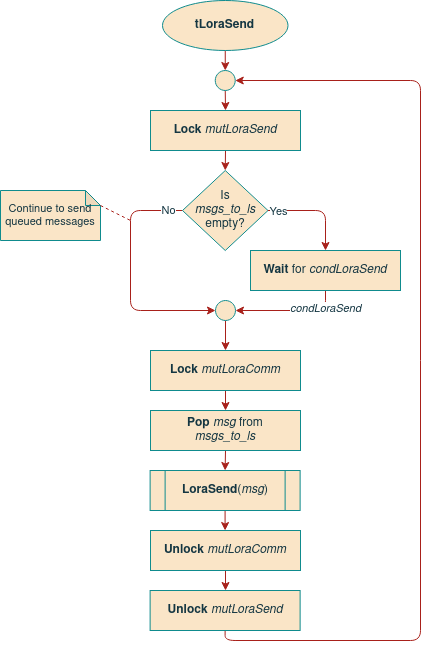
\includegraphics[width=.8\textwidth]{09sw_specification/gwtLoraSend}
%	\caption{Flowchart: Gateway tLoraSend.}
%	\label{fig:gwtLoraSend}
%\end{figure}

%\clearpage
%\myparagraph{tTCPSend}
%
%This task, presented in figure \ref{fig:gwtTCPSend}, is responsible for sending all the messages sent by the local systems to the remote system, being received by in the task \textit{tLoraRecv}. It uses two mutexes: \textit{mutTCPSend} associated with the condition variable \textit{condTCPSend}, that synchronizes the insertion and removal of the messages from the vector \textit{msgs\_to\_rs}; and \textit{mutTCPComm}, to protect the communications send and receive.
%
%When there are no messages to send to the remote system, i.e, the messages vector \textit{msgs\_to\_rs} is empty, the task enters a sleep state, waiting for \textit{condTCPSend} to be notified by the task receiving messages from the local systems. When messages are received, the vector \textit{msgs\_to\_rs} is not empty, and one can lock the mutex \textit{mutTCPSend} in order to pop a message from the vector. After that, one can send the message via TCP/IP communication protocol, protecting the communication with the mutex \textit{mutTCPComm}.
%
%\begin{figure}[H]
%	\centering
%	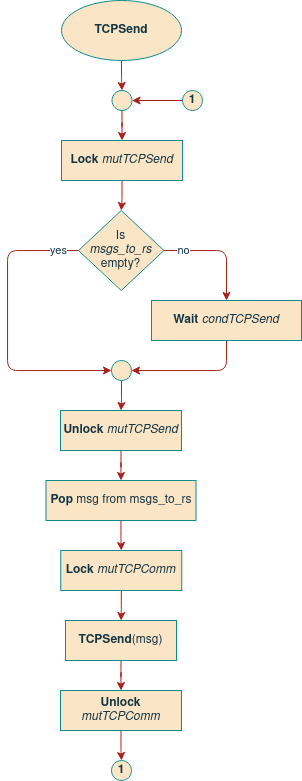
\includegraphics[width=.52\textwidth]{09sw_specification/gwtTCPSend}
%	\caption{Flowchart: Gateway tTCPSend.}
%	\label{fig:gwtTCPSend}
%\end{figure}

\myparagraph{tTCPRecv}
This task, presented in figure \ref{fig:gwtTCPRecv}, is responsible for receiving the messages sent by the remote system to the local systems. Unlike the \textit{tsend} tasks, this thread never enters the sleep state because we can receive a message at any moment. If it is received a message, then one can push the message to the messages vector in LoraComm, signaling its thread to send the message, via LoRa communication

\begin{figure}[H]
	\centering
	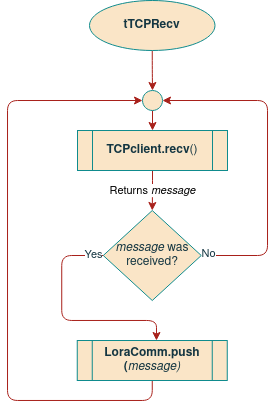
\includegraphics[width=.5\textwidth]{09sw_specification/GwtTCPRecv}
	\caption{Flowchart: Gateway tTCPRecv.}
	\label{fig:gwtTCPRecv}
\end{figure}

%%**********************************************************
\clearpage
\subsection{Start-up Process}
In figure \ref{fig:bootGateway} is shown the start-up process for the gateway. When booting up, the gateway creates the TCPclient and the LoraComm objects, initializing the peripherals needed for the gateway to communicate with the local systems and the remote server. After this the threads are created and both objects begin running their threads for receiving messages.

\begin{figure}[H]
	\centering
	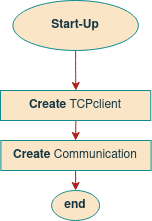
\includegraphics[width=.3\textwidth]{09sw_specification/bootGw}
	\caption{Start-Up Process: Gateway.}
	\label{fig:bootGateway}
\end{figure}

%%**********************************************************
%\subsection{Shutdown Process}
